\section{Auswertung}
\label{sec:Auswertung}
\subsection{Charakteristik des Zählrohrs} % (fold)
\label{sub:charakteristik_aus}

Die Messung wird nach \autoref{sub:charakteristik_durch} durchgeführt. Die Messwerte zu Spannung, Stromstärke und die Zählrate, sowie der Fehler
der Zählrate werden in
\autoref{tab:tab1} aufgetragen.
$N$ ist hierbei schon umgerechnet in Impulse pro Sekunde und der Fehler wird nach der Formel
\begin{align*}
  \Delta N &= \sqrt{N} 
\end{align*}
bestimmt.
\begin{table}[H]
  \centering
  \caption{Messwerte zur bestimmung der Charakteristik des Zählrohrs.}
  \label{tab:tab1}
  \sisetup{table-format=3.2}
  \begin{tabular}{S[table-format=3.0]S[table-format=1.1]S@{${}\pm{}$}S[table-format=2.2]}
  \toprule
   {$U\mathbin{/} \si{\volt}$} &{$ I \mathbin{/} \si{\micro\ampere}$} & \multicolumn{2}{c}{$N \mathbin{/} \frac{Impulse}{\si{\second}}$} \\
  \midrule 
   320 & 0.2 &  106.08 & 10.30 \\
   330 & 0.2 &  109.25 & 10.45 \\
   340 & 0.2 &  109.52 & 10.47 \\
   350 & 0.2 &  110.15 & 10.50 \\
   360 & 0.2 &  111.33 & 10.55 \\ 
   370 & 0.2 &  113.85 & 10.67 \\
   380 & 0.2 &  111.55 & 10.56 \\ 
   390 & 0.2 &  112.40 & 10.60 \\
   400 & 0.2 &  114.37 & 10.69 \\ 
   410 & 0.2 &  111.65 & 10.57 \\
   420 & 0.2 &  113.35 & 10.65 \\ 
   430 & 0.3 &  112.92 & 10.63 \\
   440 & 0.3 &  113.75 & 10.67 \\ 
   450 & 0.3 &  111.25 & 10.55 \\
   460 & 0.4 &  113.18 & 10.64 \\
   470 & 0.4 &  110.13 & 10.49 \\
   480 & 0.4 &  115.18 & 10.73 \\ 
   490 & 0.4 &  114.25 & 10.69 \\
   500 & 0.4 &  115.50 & 10.75 \\ 
   510 & 0.4 &  113.17 & 10.64 \\
   520 & 0.4 &  112.77 & 10.62 \\
   530 & 0.5 &  114.62 & 10.71 \\
   540 & 0.5 &  113.18 & 10.64 \\ 
   550 & 0.5 &  114.90 & 10.72 \\
   560 & 0.5 &  114.75 & 10.71 \\ 
   570 & 0.6 &  115.30 & 10.74 \\
   580 & 0.6 &  115.40 & 10.74 \\ 
   590 & 0.6 &  112.48 & 10.61 \\
   600 & 0.6 &  117.58 & 10.84 \\ 
   610 & 0.6 &  116.65 & 10.80 \\
   620 & 0.7 &  116.95 & 10.81 \\
   630 & 0.7 &  118.35 & 10.88 \\
   640 & 0.7 &  116.77 & 10.81 \\
   650 & 0.7 &  116.97 & 10.81 \\
   660 & 0.6 &  116.48 & 10.79 \\
   670 & 0.7 &  115.98 & 10.77 \\ 
   680 & 0.7 &  117.95 & 10.86 \\
   690 & 0.8 &  119.42 & 10.93 \\
   700 & 0.8 &  120.02 & 10.96 \\
  \bottomrule
  \end{tabular}
\end{table}

Aus den Messwerten wird die Zählrohrcharakteristik graphisch in \autoref{fig:plot1} dargestellt, also die Zählrate N gegenüber der Spannung aufgetragen.
Um den Plateauanstieg zu bestimmen wird zudem mithilfe der Pythonmodule Matplotlib\cite{matplotlib}, Scipy\cite{scipy}, Uncertainties\cite{uncertainties}
und Numpy\cite{numpy} eine Ausgleichsgerade nach $N= aU+b$ bestimmt.
\begin{figure}[H]
  \centering
  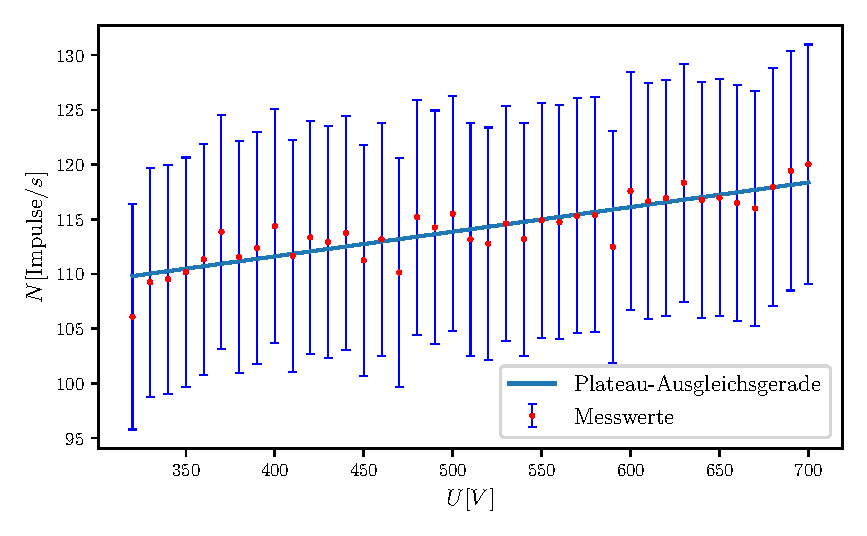
\includegraphics{build/plot1.pdf}
  \caption {Graphische Darstellung der Zählrohrcharakteristik mit Messwerten aus \autoref{tab:tab1}.}
  \label{fig:plot1}
\end{figure}

Die Parameter der linearen Regression betragen
\begin{align*}
  a &= (0.0225 \pm 0.0022)\si{\per\volt}\\
  b &= (102.60 \pm 1.13)\si{\per\second}
\end{align*}

Der relative Plateauanstieg wird zu
\begin{align*}
    a_\text{rel} &= \left( \frac{N(U=\SI{700}{\volt})}{N(U=\SI{320}{\volt})} - 1 \right) \cdot \frac{\SI{100}{\volt}}{(700-320)\:\si{\volt}} \cdot 100 \\
             &= (3.46 \pm 3.97)\si{\percent\per100\volt}
\end{align*}
bestimmt.

\subsection{Totzeit des Zählrohrs}
\label{sub:totzeit_aus}

Wie in \autoref{sub:totzeit_durch} beschrieben, wird die Totzeit des Zählrohrs auf zwei verschiedene Arten bestimmt.







